% FAR Explainer Figure - Standalone TikZ
% Compile with: pdflatex far_explainer.tex

\documentclass[tikz,border=5pt]{standalone}
\usepackage{tikz}
\usetikzlibrary{calc,3d,positioning}

\begin{document}

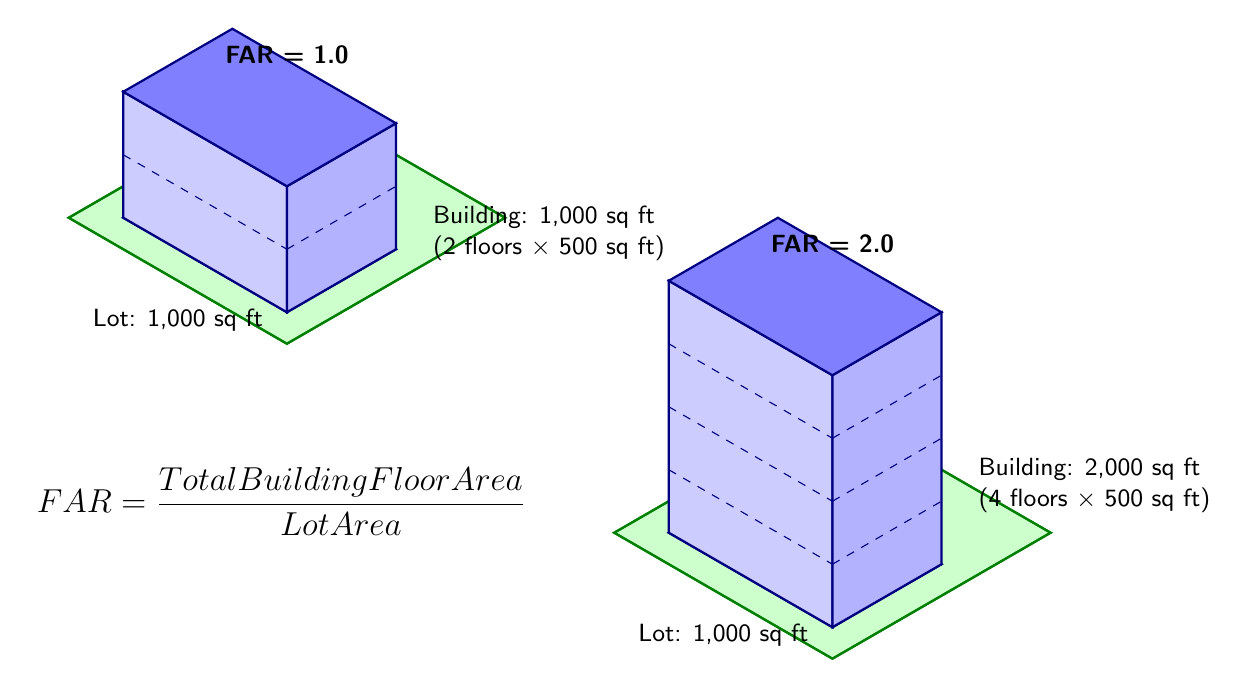
\begin{tikzpicture}[
    scale=0.8,
    % Isometric projection angles
    x={(0.866cm,-0.5cm)},
    y={(0.866cm,0.5cm)},
    z={(0cm,1cm)},
    % Styles
    lot/.style={fill=green!20, draw=green!50!black, thick},
    building/.style={fill=blue!30, draw=blue!50!black, thick},
    building top/.style={fill=blue!50, draw=blue!50!black, thick},
    building side/.style={fill=blue!20, draw=blue!50!black, thick},
    label style/.style={font=\small\sffamily},
]

% =====================================================
% LEFT PANEL: FAR = 1 (2-story building at 50% coverage)
% =====================================================
\begin{scope}[shift={(-5,0,0)}]
    % Lot (4x4 base)
    \fill[lot] (0,0,0) -- (4,0,0) -- (4,4,0) -- (0,4,0) -- cycle;
    \draw[green!50!black, thick] (0,0,0) -- (4,0,0) -- (4,4,0) -- (0,4,0) -- cycle;
    
    % Building footprint: 2x4 = 8 sq units (50% of 16 sq unit lot)
    % 2 stories, each floor = 8 sq units, total = 16 sq units
    % FAR = 16/16 = 1
    
    % Building base (front-left position)
    \def\bx{0.5} \def\by{0.5} \def\bw{3} \def\bd{2} \def\bh{2}
    
    % Bottom face (floor)
    \fill[building] (\bx,\by,0) -- (\bx+\bw,\by,0) -- (\bx+\bw,\by+\bd,0) -- (\bx,\by+\bd,0) -- cycle;
    
    % Front face
    \fill[building side] (\bx,\by,0) -- (\bx+\bw,\by,0) -- (\bx+\bw,\by,\bh) -- (\bx,\by,\bh) -- cycle;
    
    % Right face
    \fill[building] (\bx+\bw,\by,0) -- (\bx+\bw,\by+\bd,0) -- (\bx+\bw,\by+\bd,\bh) -- (\bx+\bw,\by,\bh) -- cycle;
    
    % Top face
    \fill[building top] (\bx,\by,\bh) -- (\bx+\bw,\by,\bh) -- (\bx+\bw,\by+\bd,\bh) -- (\bx,\by+\bd,\bh) -- cycle;
    
    % Floor line (showing 2 stories)
    \draw[blue!50!black, dashed] (\bx,\by,1) -- (\bx+\bw,\by,1);
    \draw[blue!50!black, dashed] (\bx+\bw,\by,1) -- (\bx+\bw,\by+\bd,1);
    
    % Labels
    \node[label style, below] at (2,0,-0.3) {Lot: 1,000 sq ft};
    \node[label style, above] at (2,2,\bh+0.3) {\textbf{FAR = 1.0}};
    
    % Building area annotation
    \node[label style, right, align=left] at (4.5,2,1) {Building: 1,000 sq ft\\(2 floors $\times$ 500 sq ft)};
\end{scope}

% =====================================================
% RIGHT PANEL: FAR = 2 (4-story building at 50% coverage)
% =====================================================
\begin{scope}[shift={(5,0,0)}]
    % Lot (4x4 base)
    \fill[lot] (0,0,0) -- (4,0,0) -- (4,4,0) -- (0,4,0) -- cycle;
    \draw[green!50!black, thick] (0,0,0) -- (4,0,0) -- (4,4,0) -- (0,4,0) -- cycle;
    
    % Building: same footprint but 4 stories
    % FAR = 32/16 = 2
    
    \def\bx{0.5} \def\by{0.5} \def\bw{3} \def\bd{2} \def\bh{4}
    
    % Bottom face (floor)
    \fill[building] (\bx,\by,0) -- (\bx+\bw,\by,0) -- (\bx+\bw,\by+\bd,0) -- (\bx,\by+\bd,0) -- cycle;
    
    % Front face
    \fill[building side] (\bx,\by,0) -- (\bx+\bw,\by,0) -- (\bx+\bw,\by,\bh) -- (\bx,\by,\bh) -- cycle;
    
    % Right face
    \fill[building] (\bx+\bw,\by,0) -- (\bx+\bw,\by+\bd,0) -- (\bx+\bw,\by+\bd,\bh) -- (\bx+\bw,\by,\bh) -- cycle;
    
    % Top face
    \fill[building top] (\bx,\by,\bh) -- (\bx+\bw,\by,\bh) -- (\bx+\bw,\by+\bd,\bh) -- (\bx,\by+\bd,\bh) -- cycle;
    
    % Floor lines (showing 4 stories)
    \foreach \h in {1,2,3} {
        \draw[blue!50!black, dashed] (\bx,\by,\h) -- (\bx+\bw,\by,\h);
        \draw[blue!50!black, dashed] (\bx+\bw,\by,\h) -- (\bx+\bw,\by+\bd,\h);
    }
    
    % Labels
    \node[label style, below] at (2,0,-0.3) {Lot: 1,000 sq ft};
    \node[label style, above] at (2,2,\bh+0.3) {\textbf{FAR = 2.0}};
    
    % Building area annotation
    \node[label style, right, align=left] at (4.5,2,2) {Building: 2,000 sq ft\\(4 floors $\times$ 500 sq ft)};
\end{scope}

% Title/formula at bottom
\node[font=\large\sffamily, align=center] at (0,-1,-1.5) {
    $\displaystyle \text{FAR} = \frac{\text{Total Building Floor Area}}{\text{Lot Area}}$
};

\end{tikzpicture}

\end{document}
